\documentclass[a4paper]{article}
\usepackage{polski}
\usepackage[english,polish]{babel}
\usepackage[utf8]{inputenc}
\usepackage[T1]{fontenc}
\usepackage{amsmath}
\usepackage{graphicx}
\usepackage{listings}
\usepackage{color}
\usepackage{indentfirst}
\usepackage{float}

% Mniejsze marginesy
\addtolength{\textwidth}{3cm}
\addtolength{\hoffset}{-1.5cm}
\addtolength{\textheight}{3cm}
\addtolength{\voffset}{-1.5cm}

% Odstęp po akapicie
\setlength{\parskip}{1ex plus 0.5ex minus 0.5ex}

\begin{document}

\begin{titlepage}

\newcommand{\HRule}{\rule{\linewidth}{0.5mm}}

\center

\textsc{\large Politechnika Wrocławska}\\[4cm] 

\HRule \\[0.6cm]
{\huge \bfseries Rozległe sieci komputerowe}\\[0.4cm] 
\textsc{\Large projekt}\\[0.4cm]

{\textsc{\large termin zajęć: poniedziałek 13:15}}\\[1.0cm]

\begin{minipage}{0.4\textwidth}
	\begin{flushleft} \large
		\emph{Autorzy:}\\[0.1cm]
		Damian \textsc{Korzekwa}, 226132
        
        Rafał \textsc{Bukowski}, 226156
	\end{flushleft}
\end{minipage}
~
\begin{minipage}{0.5\textwidth}
	\begin{flushright} \large
		\emph{Prowadzący:} \\[0.1cm]
		prof. dr hab. inż. Andrzej \textsc{Kasprzak}
	\end{flushright}
\end{minipage}\\[1cm]

\vfill

{\large Wrocław 2018}

\end{titlepage}

\tableofcontents
\newpage

%%%%%%%%%%%%%%%%%%%%%%%%%%%%%%%%%%%%%%%%%%%%%%%%%%%%%%
\section{Założenia projektowe}

\subsection{Zadanie do wykonania}

Główne zadanie projektowe polega na zaprojektowaniu sieci rozległej, w której średnie opóźnienie podczas przesyłania pakietu nie było większe niż 0.7s/pakiet.

\subsection{Podstawowe założenia}

\begin{itemize}
	\item wykorzystywane są linie transmisyjne Orange
	\item sieć ma być podłączona do Internetu
	\item klienci komunikują się z firmą poprzez sieć Internet
\end{itemize}

\subsection{Lokalizacje oddziałów}

Centrala firmy zlokalizowana jest w Opolu i jest ona jednocześnie oddziałem firmy. Pozostałe oddziały znajdują się na terenie dwóch województw: opolskiego i dolnośląskiego.

Oddziały w województwie opolskim:

\begin{itemize}
	\item Brzeg
	\item Kluczbork
\end{itemize}

Oddziały w województwie dolnośląskim:

\begin{itemize}
	\item Wrocław
    \item Wałbrzych
    \item Kłodzko
\end{itemize}

\subsection{Informacje o działaniu firmy}

Wszystkie oddziały firmy oraz centrala pracują w godzinach 9:00 - 18:00. Po godzinach pracy firmy przesyłane są raporty o sprzedaży i zamówieniach. Klienci mają możliwość składania zamówień po godzinach pracy firmy.

\subsection{Natężenie ruchu internetowego}

Natężeniu ruchu internetowego w godzinach pracy oddziałów (dziennie):

\begin{itemize}
	\item Oddział - Oddział: 10 MB
	\item Oddział - Centrala: 51.5 MB
	\item Centrala - Oddział: 20 MB
\end{itemize}

Natężenie ruchu internetowego po godzinach pracy oddziałów (dziennie):

\begin{itemize}
	\item Oddział - Oddział: 10.8 MB
	\item Oddział - Centrala: 55 MB
\end{itemize}

Łącznie wszyscy klienci generują w ciągu całego dnia ruch do Centrali 3 GB w obie strony.

%%%%%%%%%%%%%%%%%%%%%%%%%%%%%%%%%%%%%%%%%%%%%%%%%%%%%%
\section{Ogólny opis koncepcji rozwiązania}

Jako, że firma musi utrzymywać stałe połączenie z klientami, sieć powinna działać sprawnie o każdej porze i być zabezpieczona w razie awarii któregoś z dostępnych łącz. Wymagania ilości danych na dzień dla tej sieci nie są szczególnie wygórowane co pozwala przeznaczyć środki na inwestycję w bezpieczeństwo. Ważne jest też, aby zapewnić nie tylko połączenie między oddziałami i centralą ale w szczególności z Internetem, przez który klienci mogą się skomunikować z firmą.

Centrala obsługuje wszystkie i wymienia dane z pozostałymi oddziałami w większym zakresie niż one pomiędzy sobą, jest ona też miejscem z którym w głównej mierze komunikują się klienci. Oznacza to więc, że powinna mieć ona więc najszybsze i najmocniejsze łącze.

Topologia sieci jaka zostanie wykorzystana to topologia pierścienia z dodatkowymi połączeniami. Wykorzystane zostaną łącza transmisyjne Orange.

%%%%%%%%%%%%%%%%%%%%%%%%%%%%%%%%%%%%%%%%%%%%%%%%%%%%%%
\section{Dobór struktury sieci}

%%%%%%%%%%%%%%%%%%%%%%%%%%%%%%%%
\subsection{Topologia sieci}

Sieć zostanie oparta na pierścieniu z jednym dodatkowym punktem centralnym (Brzeg). Taka topologia spowoduje, że pakiety będą przechodziły maksymalnie przez dwa przełączniki pośredniczące. Spowoduje to zmniejszenie opóźnień spowodowanych przez urządzenia pośredniczące.

Topologia naniesiona na mapę, wraz z dodatkowymi połączeniami wygląda następująco:

\begin{figure}[H]
	\centering
	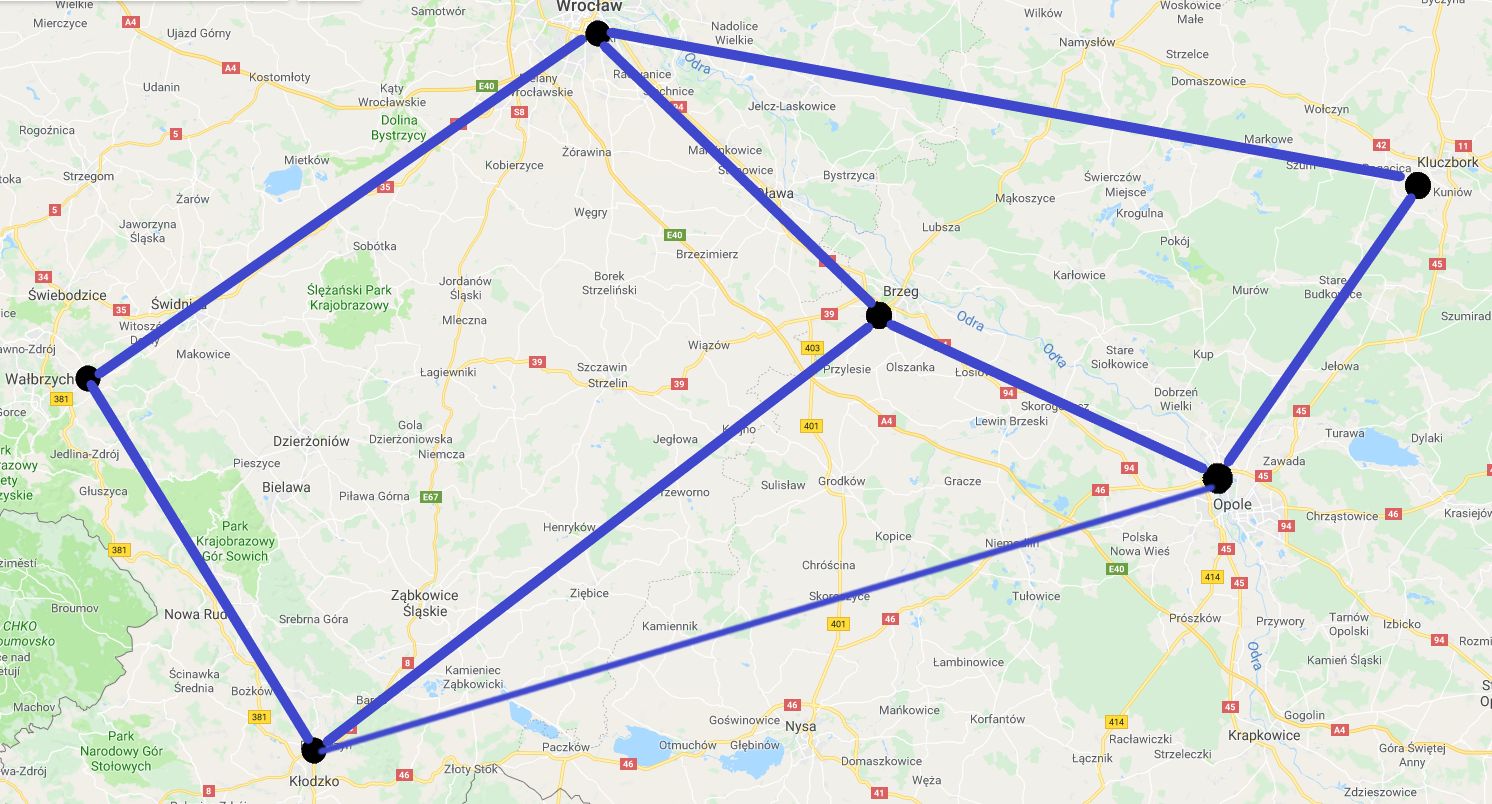
\includegraphics[width=0.75\linewidth]{mapa.png}
	\caption{Topologia sieci naniesiona na mapę}
	\label{mapa.png}
\end{figure}

Poniżej przedstawiamy schemat logiczny tej sieci:

\begin{figure}[H]
	\centering
	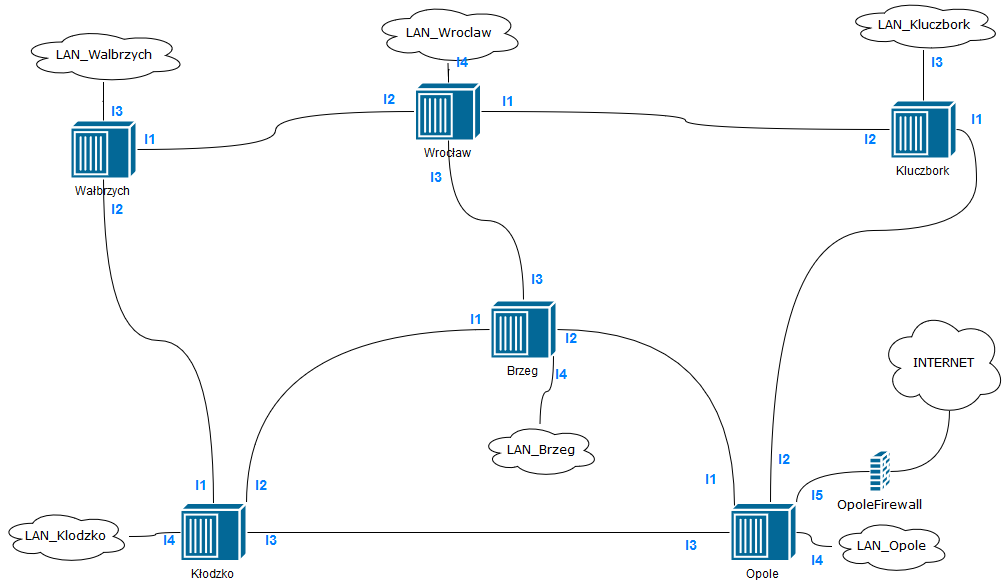
\includegraphics[width=1
    \linewidth]{diagram_sieci.png}
	\caption{Schemat logiczny sieci}
	\label{diagram_sieci.png}
\end{figure}

Odległości pomiędzy połączonymi miastami przedstawiliśmy w postaci tabeli:

\begin{table}[H]
	\centering
	\caption{Długości łączy szkieletowych}
	\label{my-label}
	\begin{tabular}{ll}
		\hline
		Połączenie & Odległość \\ \hline
		Wrocław - Wałbrzych & 65 km \\
		Wałbrzych - Kłodzko & 44 km \\
		Kłodzko - Brzeg & 74 km \\
		Brzeg - Opole & 39 km \\
		Opole - Kluczbork & 40 km \\
		Kluczbork - Wrocław & 85 km \\
		Wrocław - Brzeg & 42 km \\ 
        Kłodzko - Opole & 93 km \\
        \hline
	\end{tabular}
\end{table}

\newpage

%%%%%%%%%%%%%%%%%%%%%%%%%%%%%%%%
\subsubsection{Analiza niezawodnościowa}

Centrala musi być podłączona do Internetu cały czas, aby umożliwić komunikację z klientami. Dane, które wymienia z klientami są przekazywane dalej do oddziałów i między nimi. Jest to wiec ważne, aby awaryjność sieci był jak najniższa. 

Aby zapewnić niezawodność w sieci musimy zapewnić istnienie dwóch różnych tras z każdego węzła do pozostałych węzłów. Założenie to zostało spełnione w naszej sieci, co jest widoczne na poniższej tabelce. Pogrubione zostały nazwy miast węzłów, które są startowym i końcowym:

\begin{table}[H]
	\centering
	\caption{Możliwe trasy przesyłu danych w sieci}
	\begin{tabular}{l}
		\hline
        \textbf{Wałbrzych} (310) - \textbf{Kłodzko} (410)\\
        \textbf{Wałbrzych} (310) - Wrocław (210) - Brzeg (510) - \textbf{Kłodzko} (410)\\
        \hline
        \textbf{Wałbrzych} (310) - \textbf{Wrocław} (210) \\
		\textbf{Wałbrzych} (310) - Kłodzko (410) - Brzeg (510) - \textbf{Wrocław} (210) \\
        \hline
        \textbf{Wałbrzych} (310) - Wrocław (210) - \textbf{Brzeg} (510) \\
        \textbf{Wałbrzych} (310) - Kłodzko (410) - \textbf{Brzeg} (510) \\
        \hline
        \textbf{Wałbrzych} (310) - Kłodzko (410) - \textbf{Opole} (110) \\
        \textbf{Wałbrzych} (310) - Wrocław (210) - Brzeg (510) - \textbf{Opole} (110)  \\
        \hline
        \textbf{Wałbrzych} (310) - Wrocław (210) - \textbf{Kluczbork} (610) \\
        \textbf{Wałbrzych} (310) - Kłodzko (410) - Opole (110) - \textbf{Kluczbork} (610) \\
        \hline
        \textbf{Kłodzko} (410) - \textbf{Brzeg} (510) \\
        \textbf{Kłodzko} (410) - Opole (110) - \textbf{Brzeg} (510) \\
        \hline
        \textbf{Kłodzko} (410) - Brzeg (510) - \textbf{Wrocław} (210) \\
        \textbf{Kłodzko} (410) - Wałbrzych (310) - \textbf{Wrocław} (210) \\
        \hline
        \textbf{Kłodzko} (410) - Opole (1w.10) - \textbf{Kluczbork} (610) \\
        \textbf{Kłodzko} (410) - Brzeg (510) - Wrocław (210) - \textbf{Kluczbork} (610)\\
        \hline
        \textbf{Kłodzko} (410) - \textbf{Opole} (110) \\
        \textbf{Kłodzko} (410) - Brzeg (510) - \textbf{Opole} (110)\\
        \hline
        \textbf{Brzeg} (510) - Opole (110) - \textbf{Kluczbork} (610) \\
		\textbf{Brzeg} (510) - Wrocław (210) - \textbf{Kluczbork} (610) \\
        \hline
        \textbf{Brzeg} (510) - \textbf{Opole} (110)\\
		\textbf{Brzeg} (510) - Kłodzko (410) - \textbf{Opole} (110)\\
        \hline
        \textbf{Brzeg} (510) - \textbf{Wrocław} (210) \\ 
		\textbf{Brzeg} (510) - Kłodzko (410) - Wałbrzych (310) - \textbf{Wrocław} (210)\\
        \hline
        \textbf{Wrocław} (210) - Brzeg (510) - \textbf{Opole} (110) \\
        \textbf{Wrocław} (210) - Kluczbork (610) - \textbf{Opole} (110) \\
        \hline
        \textbf{Wrocław} (210) - \textbf{Kluczbork} (610) \\ 
        \textbf{Wrocław} (210) - Brzeg (510) - Opole (110) - \textbf{Kluczbork} (610) \\
        \hline
        \textbf{Opole} (110) - \textbf{Kluczbork} \\
        \textbf{Opole} (110) - Brzeg (510) - Wrocław (210) - \textbf{Kluczbork} (610) \\   
        \hline
	\end{tabular}
\end{table}

Na podstawie powyższych informacji z każdego oddziału oraz centrali sieć wychodzi w co najmniej dwóch kierunkach. Oznacza to, że jeżeli nastąpi awaria sieci na jednym łączu to połączenie między oddziałami zostanie zachowane poprzez zmianę trasy.

%%%%%%%%%%%%%%%%%%%%%%%%%%%%%%%%
\subsubsection{Reguła doboru tras}

\begin{table}[H]
	\centering
	\caption{Priorytety tras : Opole (110)}
	\label{xxx}
	\begin{tabular}{lll}
		\hline
		Węzeł końcowy & Interfejs & Priorytet \\
        \hline
		210 & I1 & 100 \\
		210 & I2 & 50 \\
        210 & I3 & 25 \\       
        \hline
		310 & I1 & 50 \\
		310 & I2 & 25 \\
        310 & I3 & 100 \\
        \hline
		410 & I1 & 50 \\
		410 & I2 & 25 \\
		410 & I3 & 100 \\        
        \hline
		510 & I1 & 100 \\
		510 & I2 & 25 \\
		510 & I3 & 50 \\
        \hline
		610 & I1 & 50 \\
		610 & I2 & 100 \\
		610 & I3 & 25 \\
        \hline
		110 & I4 & 100 \\
	\end{tabular}
\end{table}

\begin{table}[H]
	\centering
	\caption{Priorytety tras : Wrocław (210)}
	\label{xxx}
	\begin{tabular}{lll}
		\hline
		Węzeł końcowy & Interfejs & Priorytet \\
        \hline
		110 & I1 & 50 \\
		110 & I2 & 25 \\
		110 & I3 & 100 \\        
        \hline
		310 & I1 & 25 \\
		310 & I2 & 100 \\
		310 & I3 & 50 \\
        \hline
		410 & I1 & 25 \\
		410 & I2 & 50 \\
		410 & I3 & 100 \\       
        \hline
		510 & I1 & 25 \\
		510 & I2 & 50 \\
		510 & I3 & 100 \\
        \hline
		610 & I1 & 100 \\
		610 & I2 & 25 \\
		610 & I3 & 50 \\
        \hline
		210 & I4 & 100 \\
	\end{tabular}
\end{table}

\begin{table}[H]
	\centering
	\caption{Priorytety tras : Wałbrzych (310)}
	\label{xxx}
	\begin{tabular}{lll}
		\hline
		Węzeł końcowy & Interfejs & Priorytet \\        
        \hline
		110 & I1 & 50 \\
		110 & I2 & 100 \\
        \hline
		210 & I1 & 100 \\
		210 & I2 & 50 \\       
        \hline
		410 & I1 & 50 \\
		410 & I2 & 100 \\
        \hline
		510 & I1 & 100 \\
		510 & I2 & 50 \\
        \hline
		610 & I1 & 100 \\
		610 & I2 & 50 \\
        \hline
		310 & I4 & 100 \\
	\end{tabular}
\end{table}

\begin{table}[H]
	\centering
	\caption{Priorytety tras : Kłodzko (410)}
	\label{xxx}
	\begin{tabular}{lll}
		\hline
		Węzeł końcowy & Interfejs & Priorytet \\
        \hline
		110 & I1 & 25 \\
		110 & I2 & 50 \\
		110 & I3 & 100 \\
        \hline
		210 & I1 & 50 \\
		210 & I2 & 100 \\
		210 & I3 & 25 \\
        \hline
		310 & I1 & 100 \\
		310 & I2 & 50 \\
		310 & I3 & 25 \\
        \hline
		510 & I1 & 25 \\
		510 & I2 & 100 \\
		510 & I3 & 50 \\
        \hline
		610 & I1 & 25 \\
		610 & I2 & 50 \\
		610 & I3 & 100 \\
        \hline
		410 & I4 & 100 \\
	\end{tabular}
\end{table}

\begin{table}[H]
	\centering
	\caption{Priorytety tras : Brzeg (510)}
	\label{xxx}
	\begin{tabular}{lll}
		\hline
		Węzeł końcowy & Interfejs & Priorytet \\
        \hline
		110 & I1 & 50 \\
		110 & I2 & 100 \\
		110 & I3 & 25 \\
        \hline
		210 & I1 & 50 \\
		210 & I2 & 25 \\
		210 & I3 & 100 \\
        \hline
		310 & I1 & 50 \\
		310 & I2 & 25 \\
		310 & I3 & 100 \\
        \hline
		410 & I1 & 100 \\
		410 & I2 & 50 \\
		410 & I3 & 25 \\
        \hline
		610 & I1 & 25 \\
		610 & I2 & 100 \\
		610 & I3 & 50 \\
        \hline
		510 & I4 & 100 \\
	\end{tabular}
\end{table}

\begin{table}[H]
	\centering
	\caption{Priorytety tras : Kluczbork (610)}
	\label{xxx}
	\begin{tabular}{lll}
		\hline
		Węzeł końcowy & Interfejs & Priorytet \\
        \hline
		110 & I1 & 100 \\
		110 & I2 & 50 \\
        \hline
		210 & I1 & 50 \\
		210 & I2 & 100 \\        
        \hline
		310 & I1 & 50 \\
		310 & I2 & 100 \\        
        \hline
		410 & I1 & 100 \\
		410 & I2 & 50 \\
        \hline
		510 & I1 & 100 \\
		510 & I2 & 50 \\
        \hline
		610 & I4 & 100 \\
	\end{tabular}
\end{table}	

%%%%%%%%%%%%%%%%%%%%%%%%%%%%%%%%
\subsubsection{Wyznaczanie średniego opóźnienia pakietu}

Średnie opóźnienie pakietu (oznaczone poprzez T) można wyznaczyć używając wzoru:
$$ T = \frac{1}{\gamma} \sum_{}^{q} \frac{f(x,y)}{c(x,y) - f(x,y)} $$
gdzie:
\begin{itemize}
\item \(\gamma \) - ilość pakietów w sieci we wszystkich kanałach (pakiety/s)
\item \(f(x,y) \) - przepływ na kanale i
\item \(c(x,y) \) - przepustowość kanału i
\end{itemize}

\(\gamma \) można obliczyć dzieląc sumę przepływu na kanale przez rozmiar pakietu czyli:
$$ \gamma = \sum_{}^{q} \frac{f(x,y)}{d_{pak}} $$
gdzie \(d_{pak} = 1 kB \), a q to ilość kanałów.

Najpierw należało wyliczyć przepływy dla poszczególnych kanałów na zmianę, z tego można uzyskać przepływ w kB/s co pozwala lepiej odczytać wymagania co do szybkość przesyłu danych na konkretnym kanale.

\begin{table}[H]
	\centering
	\caption{Przepływ danych w zależności od kanałów w godzinach pracy (15h)}
	\begin{tabular}{llll}
		\hline
		Kanał & Przepływ (MB/zmianę) & Przepływ (kB/s) & Ustalona przepustowość kanału (kB/s) \\
        \hline
Wałbrzych - Kłodzko&111,5&3,52&8\\
Kłodzko - Brzeg&40&1,26&4\\
Wałbrzych - Wrocław&60&1,90&4\\
Wrocław - Brzeg&151,5&4,79&16\\
Brzeg - Opole&203&6,42&16\\
Kluczbork - Opole&131,5&4,16&16\\
Wrocław - Kluczbork&40&1,26&4\\
Kłodzko - Opole&203&6,42&16\\

        \hline
	\end{tabular}	
\end{table}

\begin{table}[H]
	\centering
	\caption{Przepływ danych w zależności od kanałów poza godzinami pracy (9h)}
	\begin{tabular}{llll}
		\hline
		Kanał & Przepływ (MB/zmianę) & Przepływ (kB/s) & Ustalona przepustowość kanału (kB/s) \\
        \hline
Wałbrzych - Kłodzko&98,2&1,86&8\\
Kłodzko - Brzeg&43,2&0,82&4\\
Wałbrzych - Wrocław&64,8&1,23&4\\
Wrocław - Brzeg&141,4&2,68&16\\
Brzeg - Opole&174,8&3,31&16\\
Kluczbork - Opole&119,8&2,27&16\\
Wrocław - Kluczbork&43,2&0,82&4\\
Kłodzko - Opole&174,8&3,31&16\\

        \hline
	\end{tabular}	
\end{table}

Dzięki powyższym tabelom można obliczyć \(\frac{f(x,y)}{d_{pak}}  \) i \(  \frac{f(x,y)}{c(x,y) - f(x,y)}\) dla poszczególnych kanałów. Wyniki w poniższych tabelach zostały zaokrąglone do dwóch miejsc po przecinku.

\begin{table}[H]
	\centering
	\caption{Przepływ danych w zależności od kanałów w godzinach pracy (9h)}
	\begin{tabular}{lll}
		\hline
		Kanał & \(\frac{f(x,y)}{d_{pak}}  \) &  \(  \frac{f(x,y)}{c(x,y) - f(x,y)}\) \\
        \hline
Wałbrzych - Kłodzko & 3,52 & 0,79 \\
Kłodzko - Brzeg & 1,26 & 0,46 \\
Wałbrzych - Wrocław & 1,90 & 0,90 \\
Wrocław - Brzeg & 4,79 & 0,43\\
Brzeg - Opole & 6,42 & 0,67\\
Kluczbork - Opole & 4,16 & 0,35 \\
Wrocław - Kluczbork & 1,26 & 0,46\\
Kłodzko - Opole & 6,42 & 0,67 \\
        \hline
	\end{tabular}	
\end{table}

Średnie opóźnienie pakietu w godzinach pracy:
$$ \gamma = \sum_{}^{q} \frac{f(x,y)}{d_{pak}} = 29,72 $$
$$ A = \sum_{}^{q} \frac{f(x,y)}{c(x,y) - f(x,y)} = 4,73 $$
$$ T = \frac{1}{\gamma} * A = 0,16 s/pakiet $$

\begin{table}[H]
	\centering
	\caption{Przepływ danych w zależności od kanałów poza godzinami pracy (15h)}
	\begin{tabular}{lll}
		\hline
		Kanał & \(\frac{f(x,y)}{d_{pak}}  \) &  \(  \frac{f(x,y)}{c(x,y) - f(x,y)}\) \\
        \hline
Wałbrzych - Kłodzko & 1,86 & 0,30 \\
Kłodzko - Brzeg & 0,82 & 0,26 \\
Wałbrzych - Wrocław & 1,23 & 0,44 \\
Wrocław - Brzeg & 2,68 & 0,20 \\
Brzeg - Opole & 3,31 & 0,26\\
Kluczbork - Opole & 2,27 & 0,17 \\
Wrocław - Kluczbork & 0,82 & 0,26\\
Kłodzko - Opole & 3,31 & 0,26 \\
        \hline
	\end{tabular}	
\end{table}

Średnie opóźnienie pakietu poza godzinami pracy:
$$ \gamma = \sum_{}^{q} \frac{f(x,y)}{d_{pak}} = 16,31 $$
$$ A = \sum_{}^{q} \frac{f(x,y)}{c(x,y) - f(x,y)} = 2,15 $$
$$ T = \frac{1}{\gamma} * A = 0,13 s/pakiet $$
	
Jak widać średnie opóźnienie pakietu wynosi 0,16 s/pakiet i 0,13 s/pakiet. Do tego mogą dojść jeszcze opóźnienia stworzone przez firewall jak i wygenerowane przez samo użycie protokołu X.25. Opóźnienia te jednak będą niższe od przyjętej granicy 0,7 s/pakiet.


%%%%%%%%%%%%%%%%%%%%%%%%%%%%%%%%
\subsubsection{Logika połączeń między portami urządzeń w oddziałach wojewódzkich}

Do potrzeb firmy wystarczające jest połączenie port-port. Jest ono dość tanie i łatwiejsze w użyciu, możliwa też jest szybsza rozbudowa sieci niż np. przy zastosowaniu agregacji portów. Najważniejsze jest jednak to, że firma ma niskie potrzeby odnośnie prędkości przesyłu danych, oszczędność więc wynikające z tego typu połączeń między urządzeniami jest widoczna.


%%%%%%%%%%%%%%%%%%%%%%%%%%%%%%%%%%%%%%%%%%%%%%%%
\section{Adresacja w sieci}
%%%%%%%%%%%%%%%%%%%%%%%%%%%%%%%%%%%%%%%%%%%%%%%%

Zdecydowaliśmy się skorzystać z protokołu X.25 dla naszej sieci. Aby użyć tego protokołu można skorzystać z adresacji X.121. Polega ona na przypisaniu każdemu z użytkowników sieci unikalnego adresu. Długość adresu wynosi 14 cyfr dziesiętnych.

Adres składa się z 4 pól:

P - znacznik międzynarodowy (1 cyfra)

DNIC - identyfikator sieci publicznej (4 cyfry) - w naszym projekcie jest to 260 1

NTN (national terminal number) składa się z 10 cyfr:
\begin{itemize}
\item PNIC - identyfikator sieci prywatnej (6 cyfr) - jest to numer przydzielany przez zewnętrzną organizację, dlatego pomijamy go i zastępujemy *
\item ETN - numer DTE w sieci prywatnej (4 cyfry)
\end{itemize}

Adresy prezentują się w następujący sposób:
260 1 ******* XY0
X - numer sieci
Y - numer węzła

\begin{table}[H]
	\centering
	\caption{Adresacja X.121}
	\begin{tabular}{lll}
		\hline
		Lp. & Użytkownik końcowy & Adres \\
        \hline
1. & LAN\_Opole & 260 1 ******* 110 \\
2. & INTERNET & 260 1 ******* 120 \\
3. & LAN\_Wroclaw & 260 1 ******* 210 \\
3. & LAN\_Walbrzych & 260 1 ******* 310 \\
4. & LAN\_Klodzko & 260 1 ******* 410 \\
5. & LAN\_Brzeg & 260 1 ******* 510 \\
6. & LAN\_Kluczbork & 260 1 ******* 610 \\
        \hline
	\end{tabular}	
\end{table}

%%%%%%%%%%%%%%%%%%%%%%%%%%%%%%%%%%%%%%%%%%%%%%%%
\section{Wykaz urządzeń}
%%%%%%%%%%%%%%%%%%%%%%%%%%%%%%%%%%%%%%%%%%%%%%%%

Poniżej znajduje się tabela z urządzeniami, których potrzebujemy do budowy niniejszego projektu sieci.

\begin{table}[H]
	\centering
	\caption{Wykaz urządzeń}
	\begin{tabular}{lll}
		\hline
        Rodzaj urządzenia & Model & Ilość \\
        \hline
        Przełącznik & X.25 Athena Switch & 6 \\
        Router & Cisco 1720 1-Port & 6 \\
        \hline
	\end{tabular}	
\end{table}

W każdym oddziale znajduje się router który służy głównie do łączenia się z Internetem w głównej mierze, aby kontaktować się z klientami. Oprócz tego znajduje się tam też przełącznik do którego podłączona jest infrastruktura danego oddziału, łączą się one też z innymi oddziałami, co zostało już wyżej zaprezentowane.


Karty katalogowe powyższych urządzeń:

http://www.develcon.com/athena.htm

http://cpham.perso.univ-pau.fr/CNA/CISCO1721/RouterOverview.pdf

\section{Literatura}

1. Andrzej Kasprzak, Sieci komputerowe z komutacją pakietów, Politechnika Wrocławska 1999r. ISBN: 83-7085-439-7

\end{document}